\documentclass[tikz,border=8pt]{standalone}
\usepackage[dvipsnames]{xcolor}
\usetikzlibrary{shapes.geometric,arrows.meta,positioning,fit,backgrounds,calc}

\begin{document}
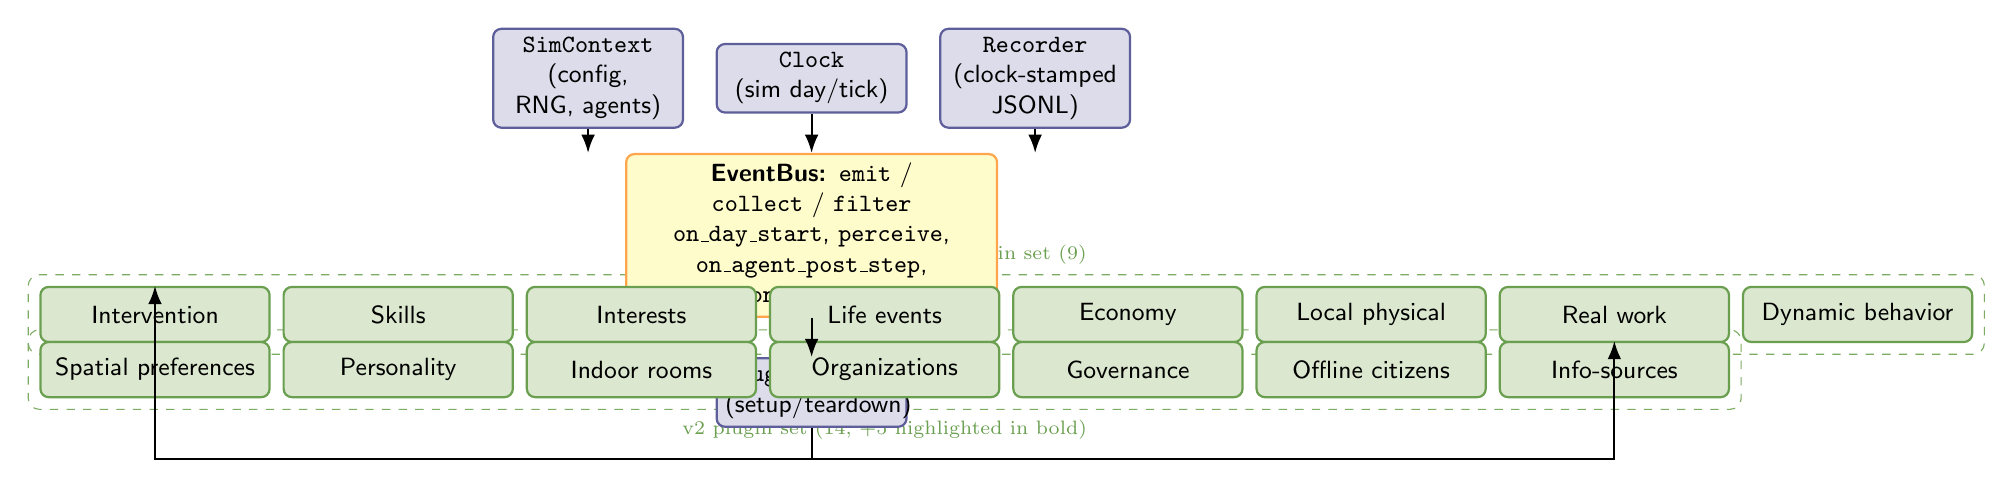
\begin{tikzpicture}[
  font=\sffamily\small,
  kernbox/.style={rectangle, draw, thick, rounded corners=3pt, align=center, minimum height=0.7cm, inner sep=3pt},
  kern/.style={kernbox, fill=MidnightBlue!15, draw=MidnightBlue!70, text width=2.2cm},
  bus/.style={kernbox, fill=yellow!20, draw=orange!70, text width=4.5cm},
  plug/.style={kernbox, fill=OliveGreen!15, draw=OliveGreen!70, text width=2.7cm},
  ar/.style={-Latex, thick},
  >={Stealth[length=2mm]}
]

% Top row: kernel
\node[kern] (ctx) at (0,0) {\texttt{SimContext}\\(config, RNG, agents)};
\node[kern, right=0.4cm of ctx] (clk) {\texttt{Clock}\\(sim day/tick)};
\node[kern, right=0.4cm of clk] (rec) {\texttt{Recorder}\\(clock-stamped JSONL)};

% Bus
\node[bus, below=0.5cm of clk] (b) {%
  \textbf{EventBus:} \texttt{emit} / \texttt{collect} / \texttt{filter}\\
  \texttt{on\_day\_start}, \texttt{perceive}, \texttt{on\_agent\_post\_step}, \texttt{on\_day\_end}};

% Registry
\node[kern, below=0.5cm of b, text width=2.2cm] (reg) {\texttt{PluginRegistry}\\(setup/teardown)};

% 14 plugins (2 rows)
\node[plug] (p1) at (-5.5,-3.0) {Intervention};
\node[plug, right=0.15cm of p1] (p2) {Skills};
\node[plug, right=0.15cm of p2] (p3) {Interests};
\node[plug, right=0.15cm of p3] (p4) {Life events};
\node[plug, right=0.15cm of p4] (p5) {Economy};
\node[plug, right=0.15cm of p5] (p6) {Local physical};
\node[plug, right=0.15cm of p6] (p7) {Real work};
\node[plug, right=0.15cm of p7] (p8) {Dynamic behavior};

\node[plug] (p9) at (-5.5,-3.7) {Spatial preferences};
\node[plug, right=0.15cm of p9] (p10) {Personality};
\node[plug, right=0.15cm of p10] (p11) {Indoor rooms};
\node[plug, right=0.15cm of p11] (p12) {Organizations};
\node[plug, right=0.15cm of p12] (p13) {Governance};
\node[plug, right=0.15cm of p13] (p14) {Offline citizens};
\node[plug, right=0.15cm of p14] (p15) {Info-sources};

% Arrows
\draw[ar] (ctx.south) -- (b.north -| ctx);
\draw[ar] (clk.south) -- (b.north -| clk);
\draw[ar] (rec.south) -- (b.north -| rec);
\draw[ar] (b) -- (reg);
\draw[ar] (reg.south) -- ++(0,-0.4) -| (p1.north);
\draw[ar] (reg.south) -- ++(0,-0.4) -| (p15.north);

% Frame around plugins
\begin{scope}[on background layer]
  \node[draw=OliveGreen!60, dashed, rounded corners=4pt, fit=(p1)(p8), inner sep=4pt, label={[OliveGreen!70, font=\scriptsize]above:{v1 plugin set (9)}}] (frame1) {};
  \node[draw=OliveGreen!60, dashed, rounded corners=4pt, fit=(p9)(p15), inner sep=4pt, label={[OliveGreen!70, font=\scriptsize]below:{v2 plugin set (14; +5 highlighted in bold)}}] (frame2) {};
\end{scope}

\end{tikzpicture}
\end{document}
